\subsection{Training on a balanced GENIE Dataset}

\noindent The solution to this imbalanced dataset problem was to pass to the model an equal number of of $\nu_\mu$, $\nu_e$ and NC events. As it was not possible to obtain more training samples for $\nu_e$ events, so the solution, as discussed previously, was to filter the the $\nu_\mu$ and NC events so that the numbers of each matched the number of $\nu_e$ events in the dataset. The balanced dataset contains 10432 $\nu_\mu$ events, 10,245 $\nu_\e$ events and 10236 $NC$ events. \medskip

\noindent For this dataset the training performance, measured by classifier accuracy and categorical cross-entropy loss, was much poorer than the training process without the filtering process to ensure equal numbers of the interaction types, which can be seen in Figures 12 and 13. The reason for this is simply that the number of training examples given to the network was fewer, and overfitting again takes place. For this reason the network was trained over 100 epochs, as a previous network trained over 200 epochs saw the performance metrics, accuracy and loss, of the network deteriorate as it trained for a longer period of time, as the network continued to overfit in such a way. \medskip

\begin{figure}[t!]
 \centering
 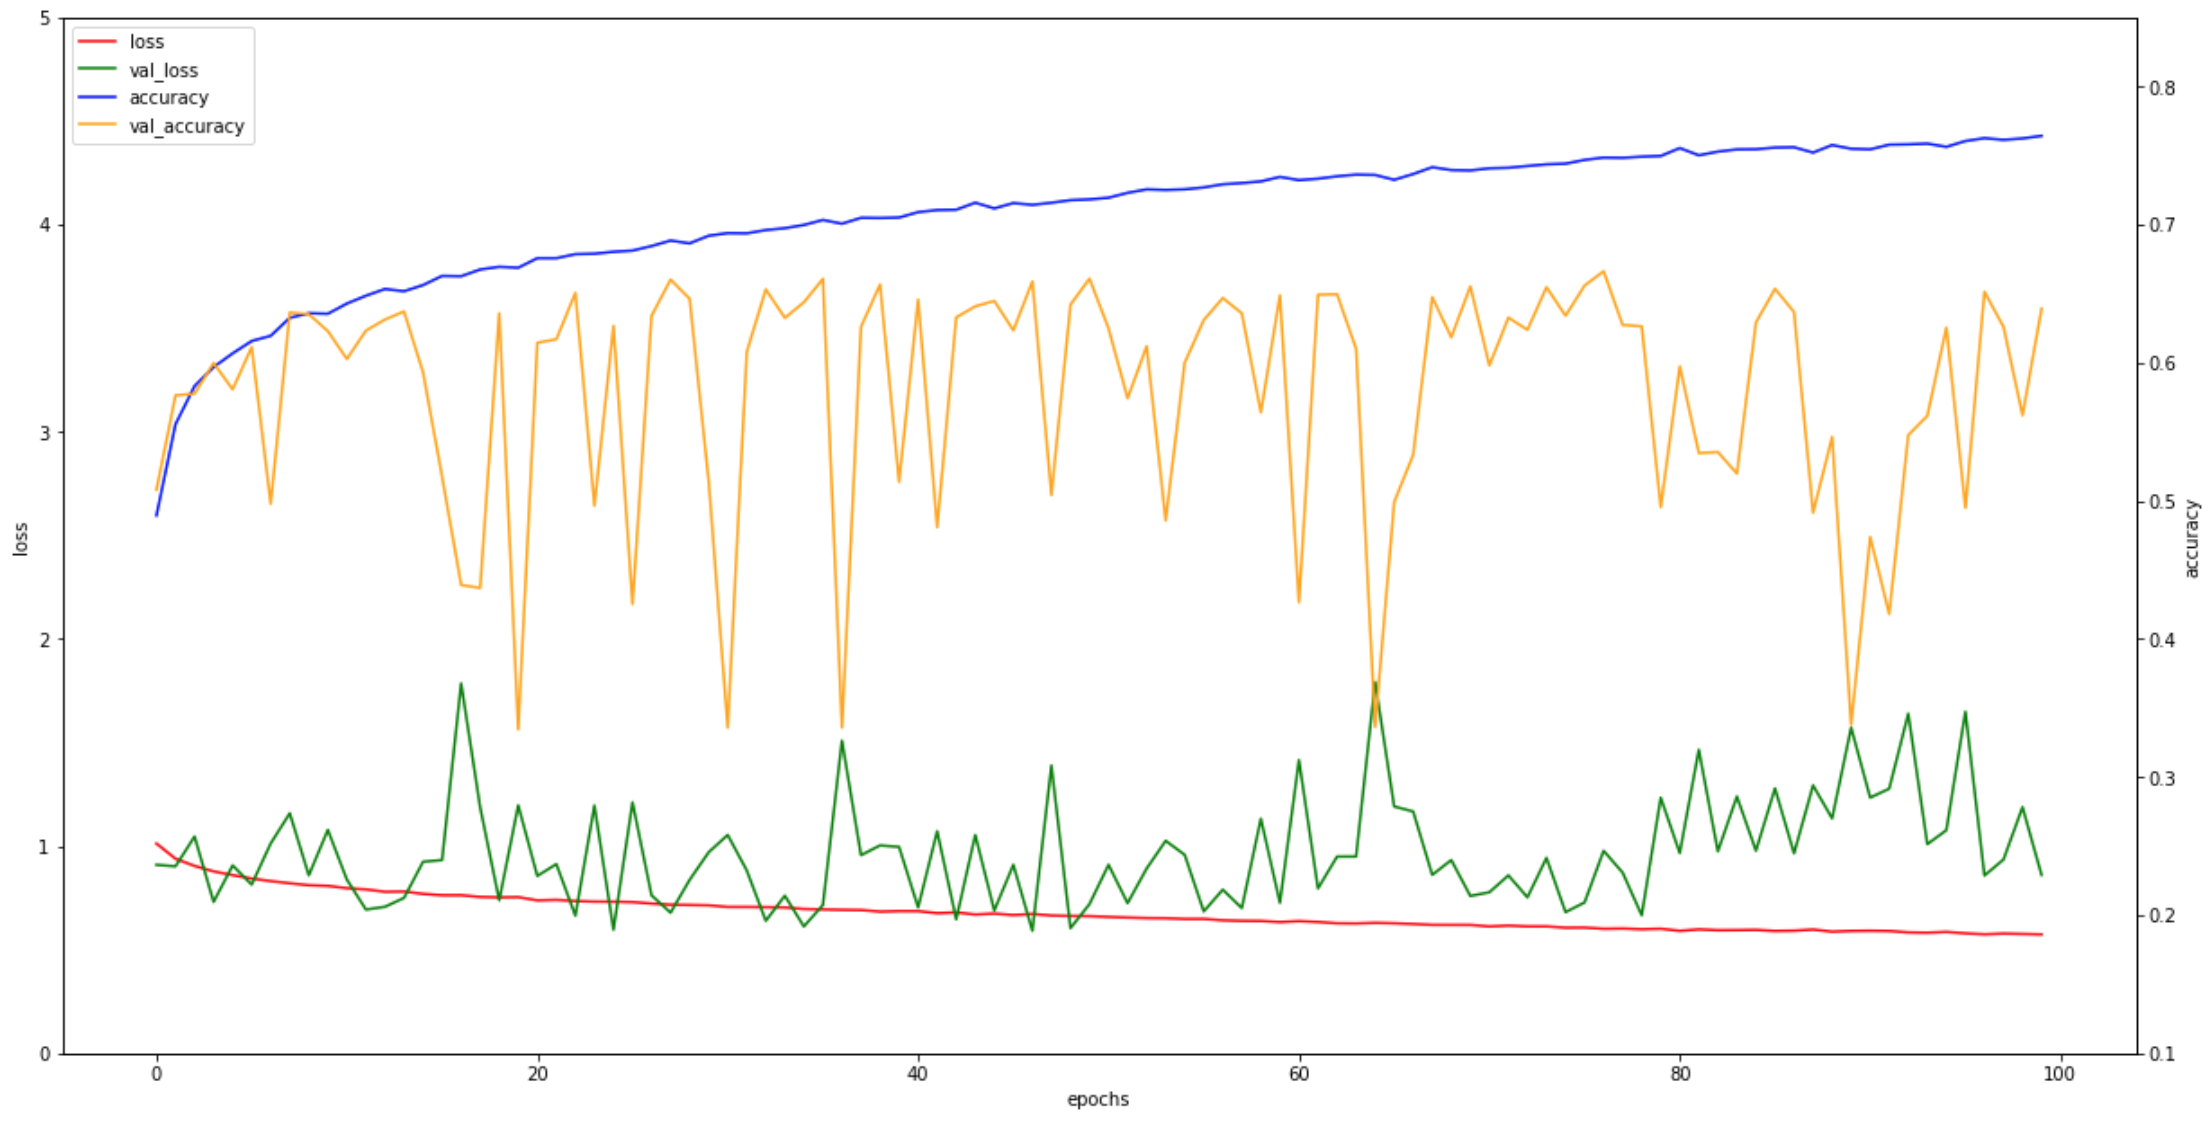
\includegraphics[width=160mm]{genie/bal_genie/bal_genie_acc.png}
 \textbf{Figure 12.} \textit{Network training and validation accuracy and loss. The network was trained over 100 epochs using only GENIE generated events, with a balanced number of each of the 3 interaction types.}
\end{figure}

\noindent This classifier, despite being trained on a smaller proportion of the data performed much better than the previous classifier by not classifying all events as the most common type.  In Figure 13 it can be seen that the $\nu_\mu$ classifier correctly classified $\nu_e$ and NC events as not $\nu_\mu$ events- something the previous classifier was unable to do as it had seen a much greater proportion of $\nu_\mu$ events than any of the others, and as a result could categorise any event as $\nu_\mu$ and be correct more often than not. The classifier is also able to correctly identify $\nu_e$ events as not $\nu_\mu$ events, and to a lesser extent the $NC$ events. \medskip

\noindent In Figure 14, which shows the $\nu_e$ classifier output, it can be seen to classify many of the the $\nu_e$ events correctly, and correctly identify the a number of $\nu_\mu$ events as not $\nu_e$ events with a large confidence. Qualitatively, it can also be seen to classify the $NC$ events as not $\nu_e$ events better than the $\nu_\mu$ classifier classifies the $NC$ events as not $\nu_\mu$. \medskip

\noindent A more quantitative method of determining the performance of a classifier is to calculate the classification purity and efficiency over the various selection cut values. Purity is the the fraction of signal events in the sample that remain after making a selection cut, and is synonymous to the accuracy of the classifier determined in the training process, for events with a output value above that cut. \medskip

\noindent The selection cuts are made with the classification confidence that is given as the final output values of the neural network. Events that are classified with a lower confidence value than the cut are not used in any further analysis, with a good classifier giving the signal events at higher confidence values if classifying them correctly. \medskip

\begin{figure}[t!]
 \centering
 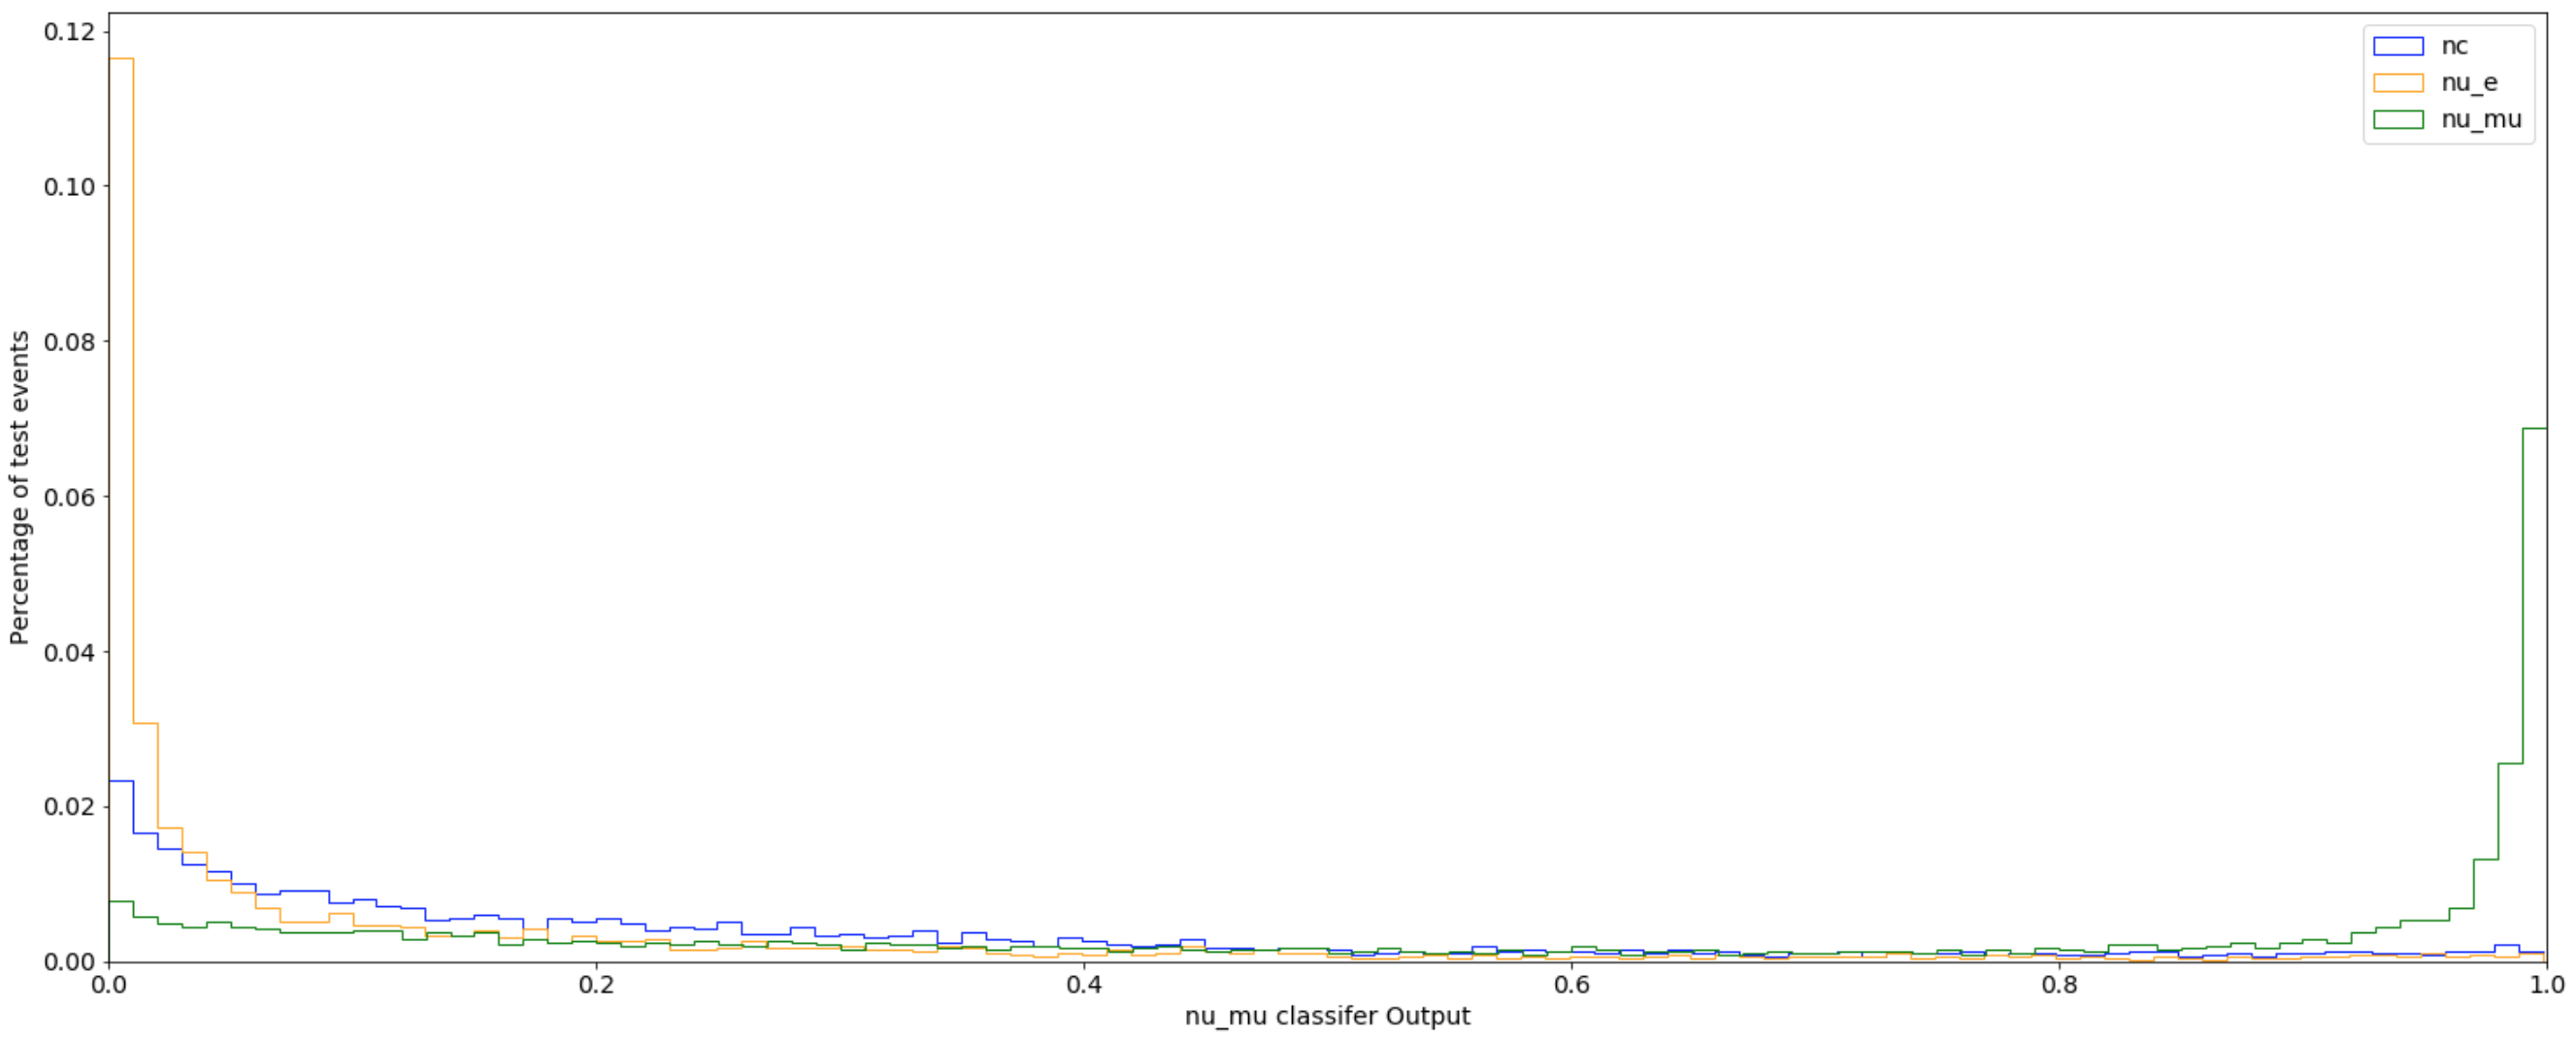
\includegraphics[width=160mm]{genie/bal_genie/bal_genie_mu.png}
 \textbf{Figure 13.} \textit{$\nu_\mu$ classification output histogram. The dataset was trained and tested using balanced GENIE only events. Figures show the probability of being classified a $\nu_\mu$ for events of all the interaction types.}
\end{figure}

\begin{figure}[t!]
 \centering
 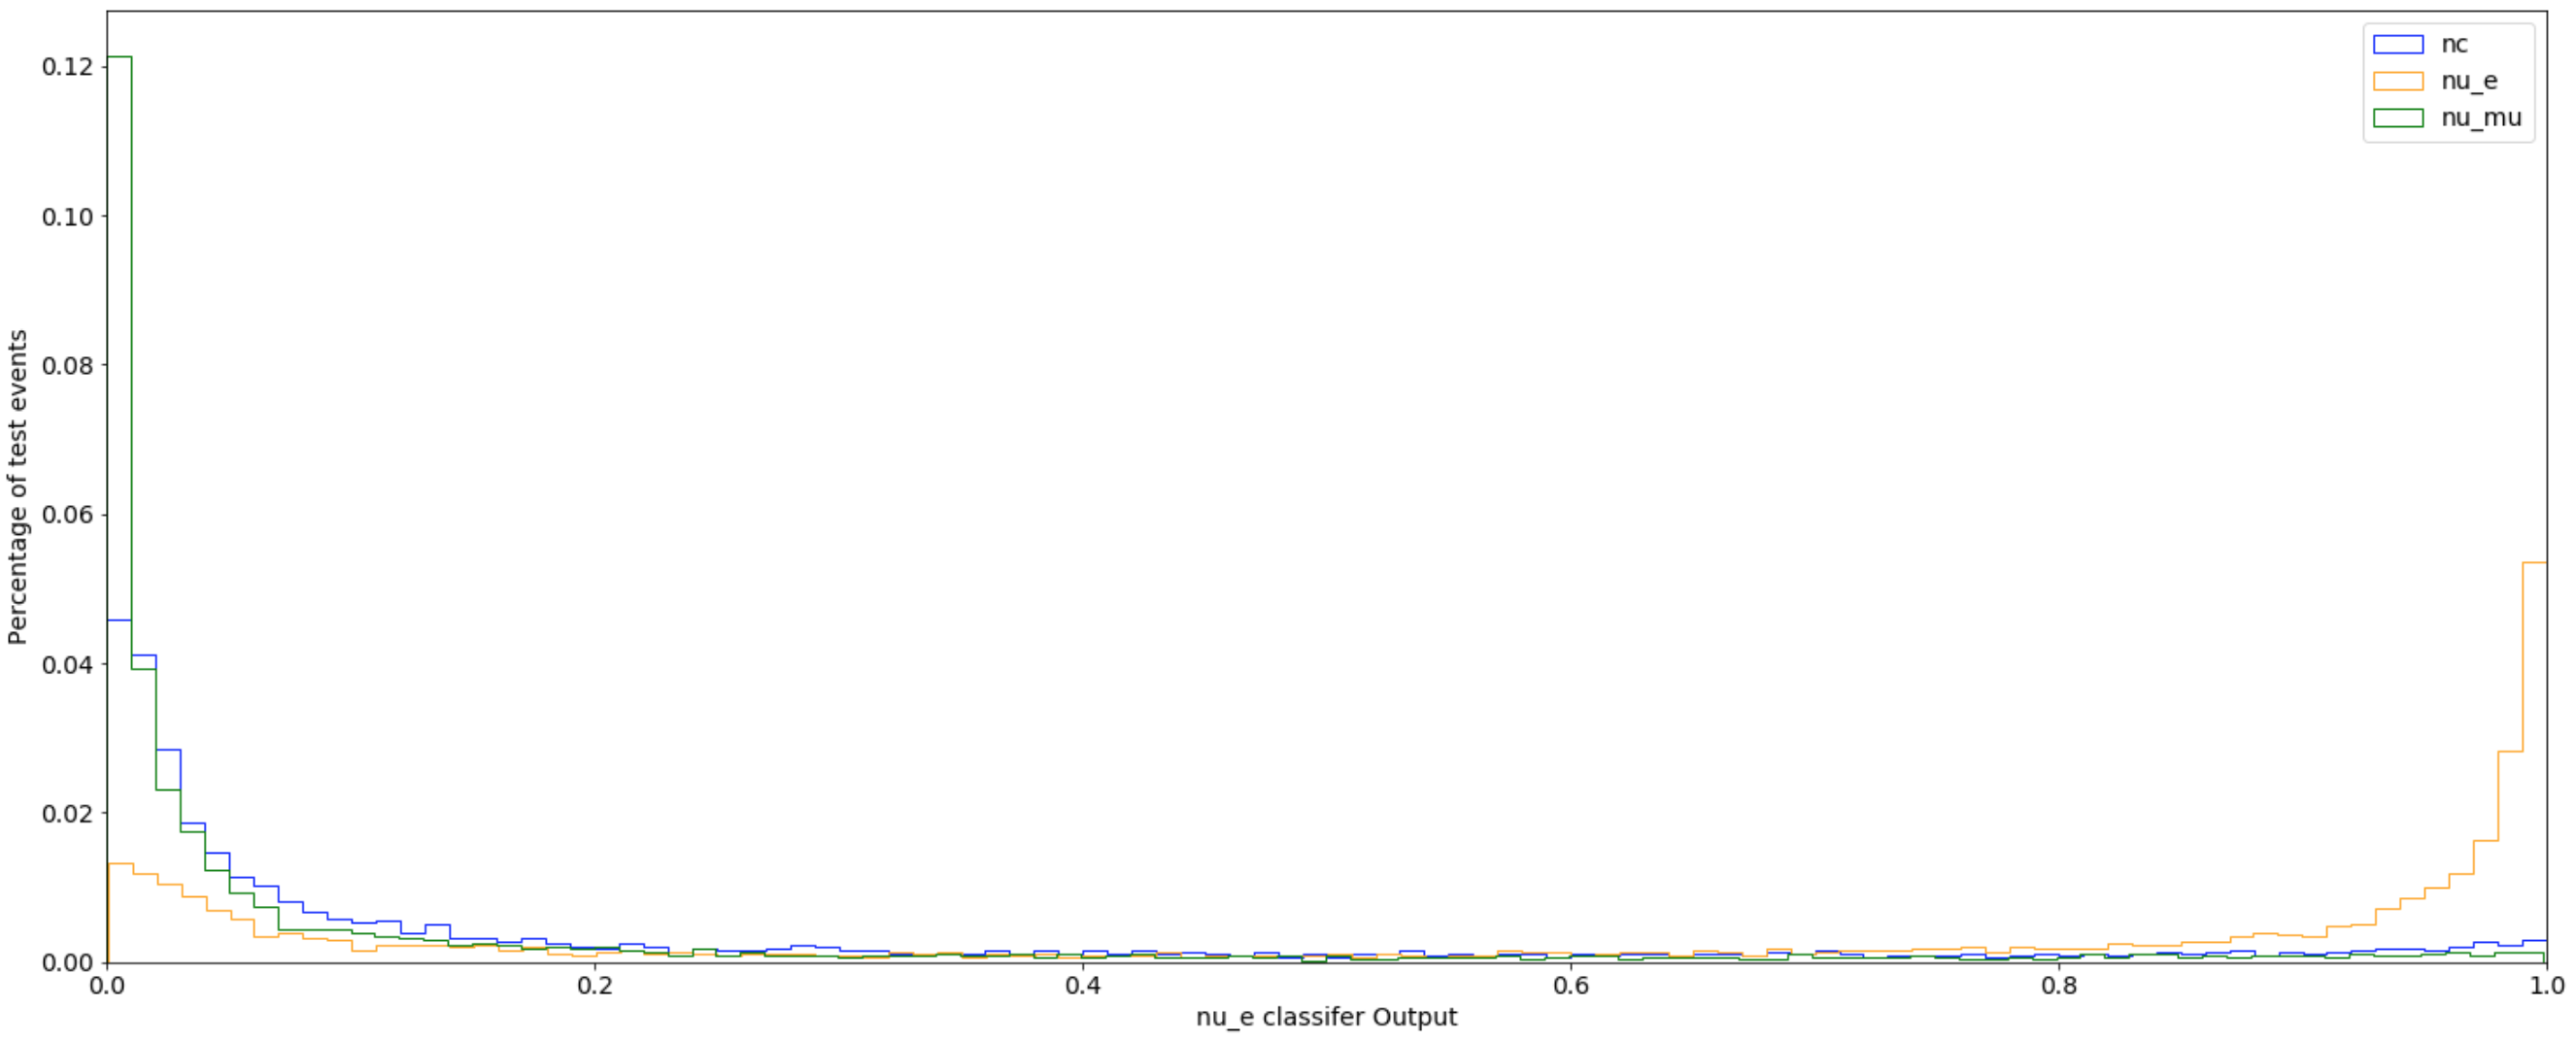
\includegraphics[width=160mm]{genie/bal_genie/bal_genie_e.png}
 \textbf{Figure 14.} \textit{$\nu_e$ classification output histogram. The dataset was trained and tested using balanced GENIE only events. Figures show the probability of being classified a $\nu_e$ for events of all the interaction types}
\end{figure}

\noindent Figure 15 shows the purity and efficiency curves for $\nu_\mu$ classification, where the signal is the $\nu_\mu$ events, and the background the $\nu_e$ and $NC$ events. At a selection cut of 0 our sample, which would contain the entire dataset, is at its most impure, as the sample contains all the events from the testing dataset, meaning the purity value will be $1/3$ given that there are an equal number of the 3 event interaction types. Scanning the confidence values, the number of $\nu_\mu$ compared to the other interaction types increases as the classifier correctly identifies $\nu_\mu$ events, until a cut of very close to 1. Here almost all of the events in the sample are $\nu_\mu$ events, and very few are $\nuFe$ or $NC$ events. This value was 0.92, and an accuracy of 92\% would correspond to a very good classifier, however it would ignore that a large number of the $\nu_\mu$ are disregarded by using a cut so high, meaning the efficiency of the classifier must be taken into account. \medskip

\begin{figure}[t!]
 \centering
 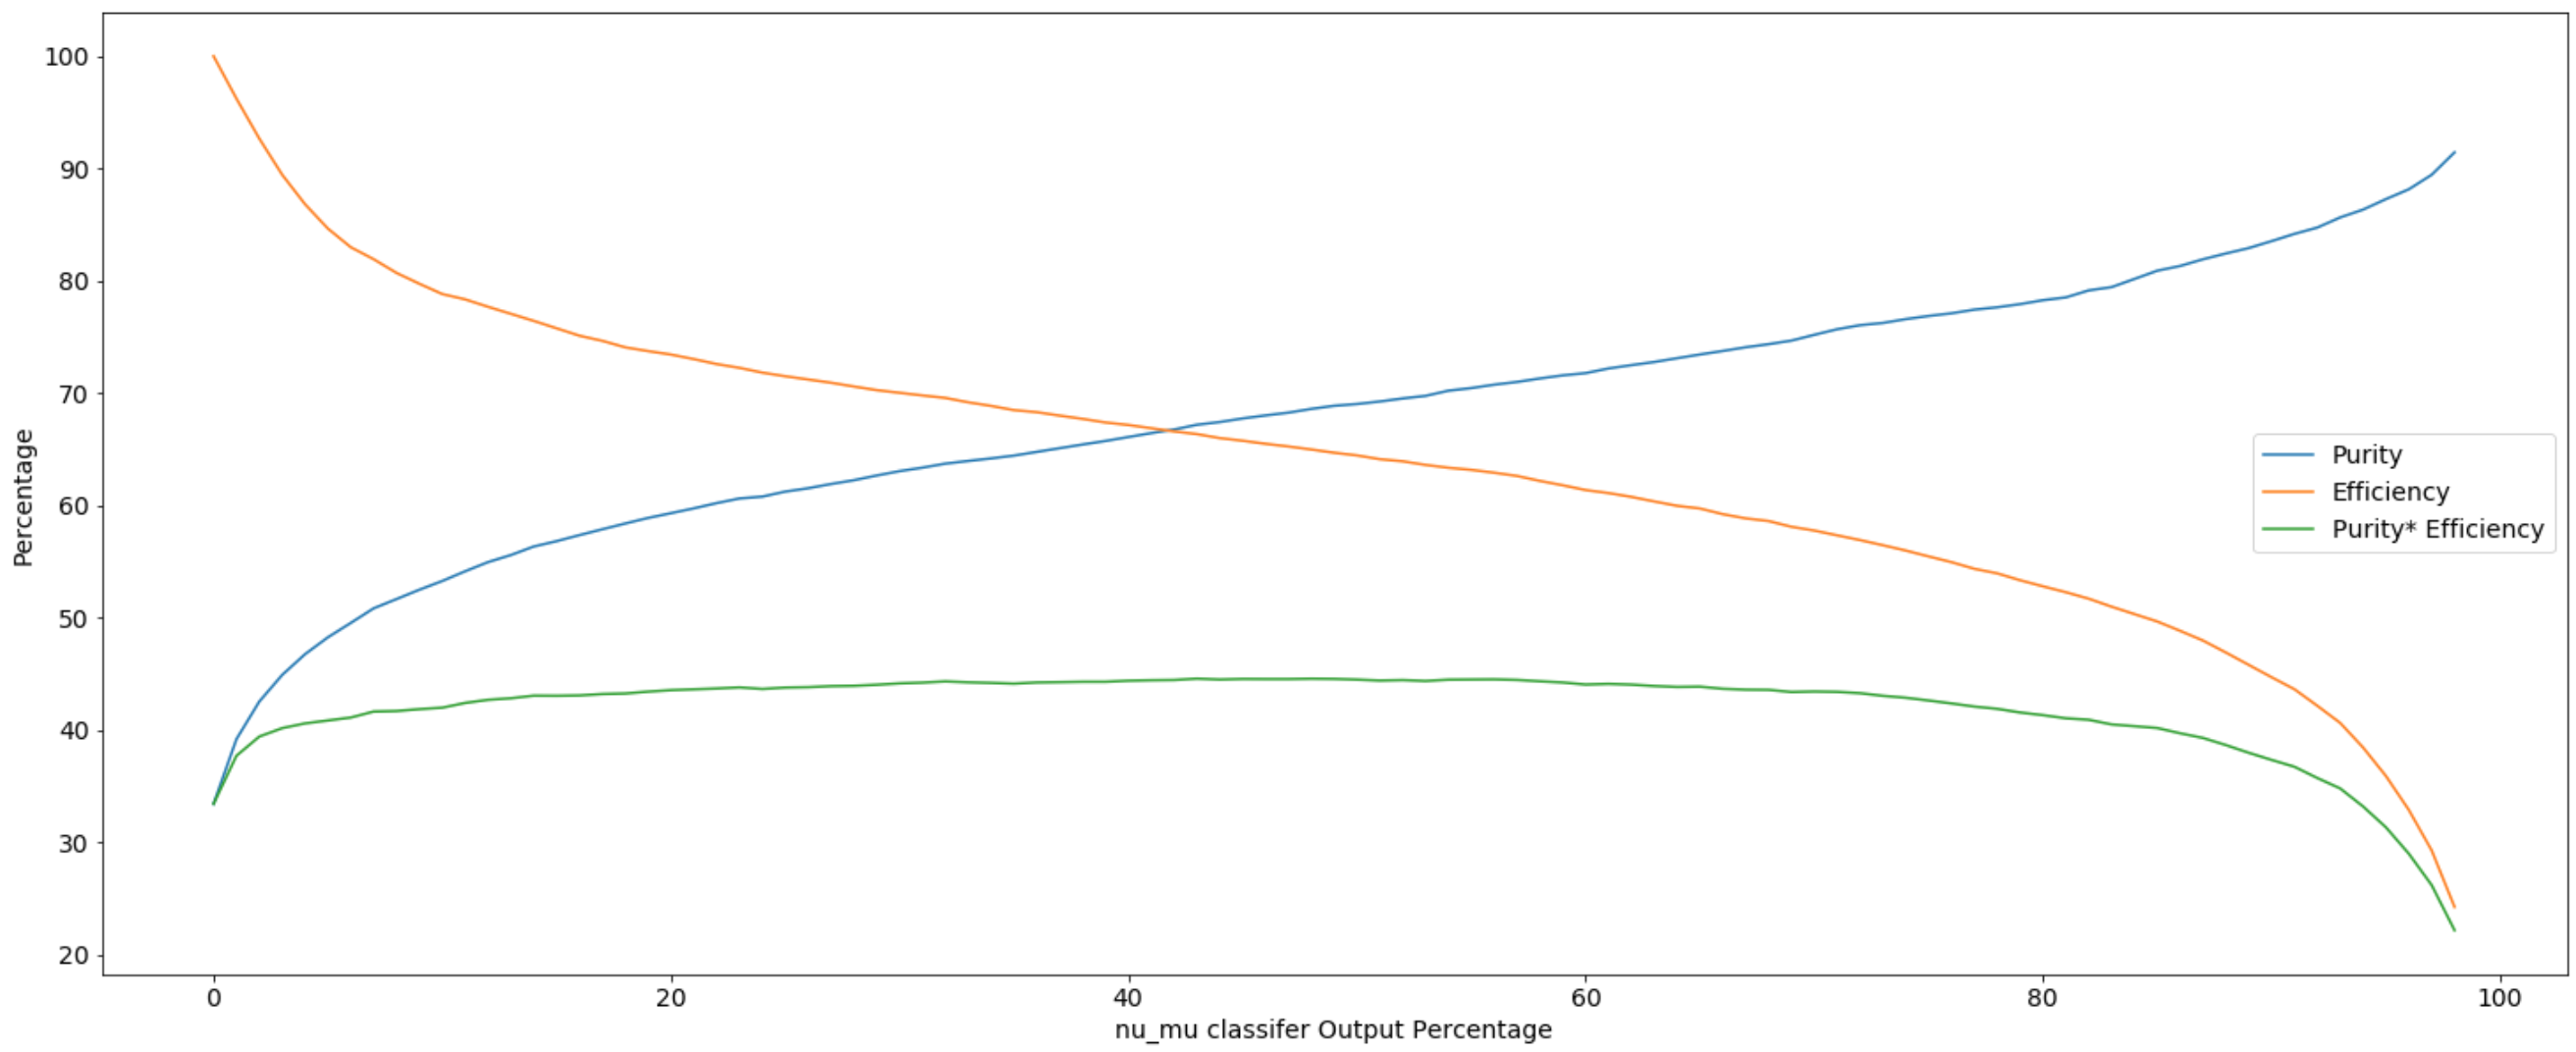
\includegraphics[width=160mm]{genie/bal_genie/bal_genie_mu_pe.png}
 \textbf{Figure 15.} \textit{Purity, efficiency and their product, curves for the $\nu_\mu$ classifier trained and tested on on a balanced GENIE dataset. The x-axis shows the confidence percentage of the network out (output multiplied by 100 to give the percentage).}
\end{figure}

\begin{figure}[t!]
 \centering
 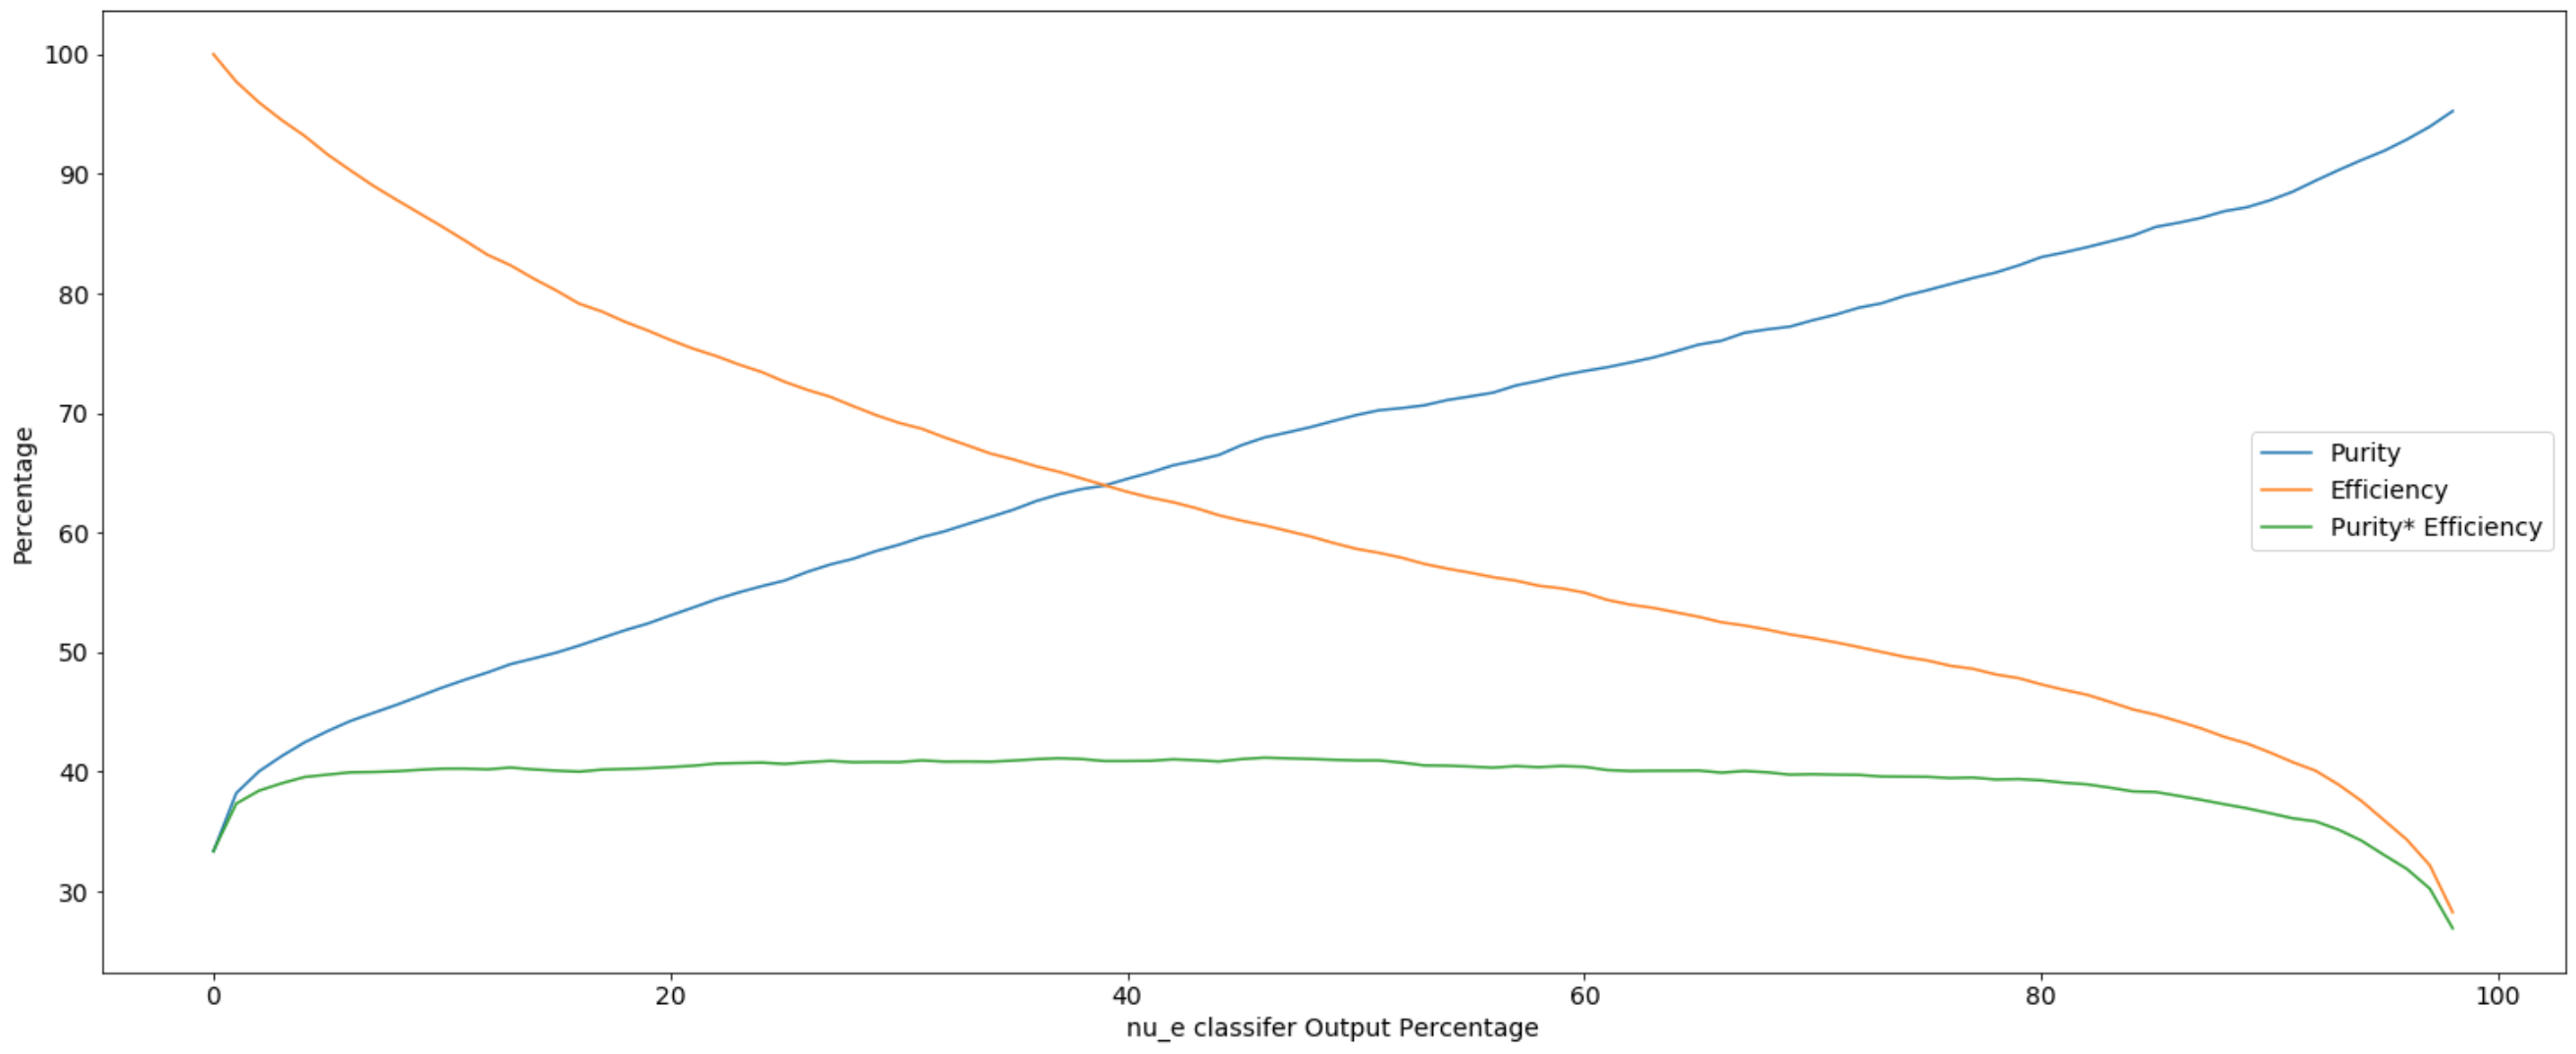
\includegraphics[width=160mm]{genie/bal_genie/bal_genie_e_pe.png}
 \textbf{Figure 16.} \textit{Purity, efficiency and their product, curves for the $\nu_e$ classifier trained and tested on a balanced GENIE dataset.}
\end{figure}

\noindent The efficiency is the fraction of the signal samples in the selected sample to the total number of signal events in the test dataset. At a low selection cut the efficiency value will be high as the most of the signal events will be contained in the selected sample. As the cut value increases, the efficiency will fall if there are signal events that are misclassified. \medskip

\noindent As the purity increases, the efficiency decreases meaning that a trade off must be made to select a correct cut value. On Figure 15, the product of purity and efficiency is also plotted, and this shows that cuts at very high and very low values will yield poor results. It is this purity efficiency curve that can be used to compare classifiers, with a better classifier having a curve with larger values, further from the X-axis.  Figure 16 shows the purity, efficiency and their product for the $\nu_e$ classifier. The $\nu_e$ classifier, performs similarly to the $\nu_\mu$ classifier, when trained on equal numbers of event integration types from the GENIE generator. 

